% Beamerで日本語を扱うときにはdocumentクラスのオプションにunicodeを指定しておく
% ここでのunicodeオプションはhyperrefパッケージに渡すためのもの

\documentclass[unicode]{beamer}


% デフォルトのLatin Modernフォントはスライド用としては細身すぎるのでLibertinusフォントに変更
\usepackage[no-math]{fontspec}
\usepackage[math-style=ISO, bold-style = ISO]{unicode-math}
\setmathfont{Libertinus Math}
\setmainfont{Libertinus Serif}
\setsansfont{Libertinus Sans}

% 日本語対応
\usepackage[ipaex]{luatexja-preset}
\renewcommand{\kanjifamilydefault}{\gtdefault}

% ムービー用パッケージ
\usepackage{multimedia}

\author{野口匠}
\institute{そのへん}
\date{2021/09/24}

\begin{document}
\begin{frame}
	\maketitle
\end{frame}

% \movie[option]{poster text}{movie file} の書式

\begin{frame}{PDF内で再生}
	\centering
	\movie[width=8cm, height=4.5cm]{%
		% ここがサムネ(テキストでも図でも可)
		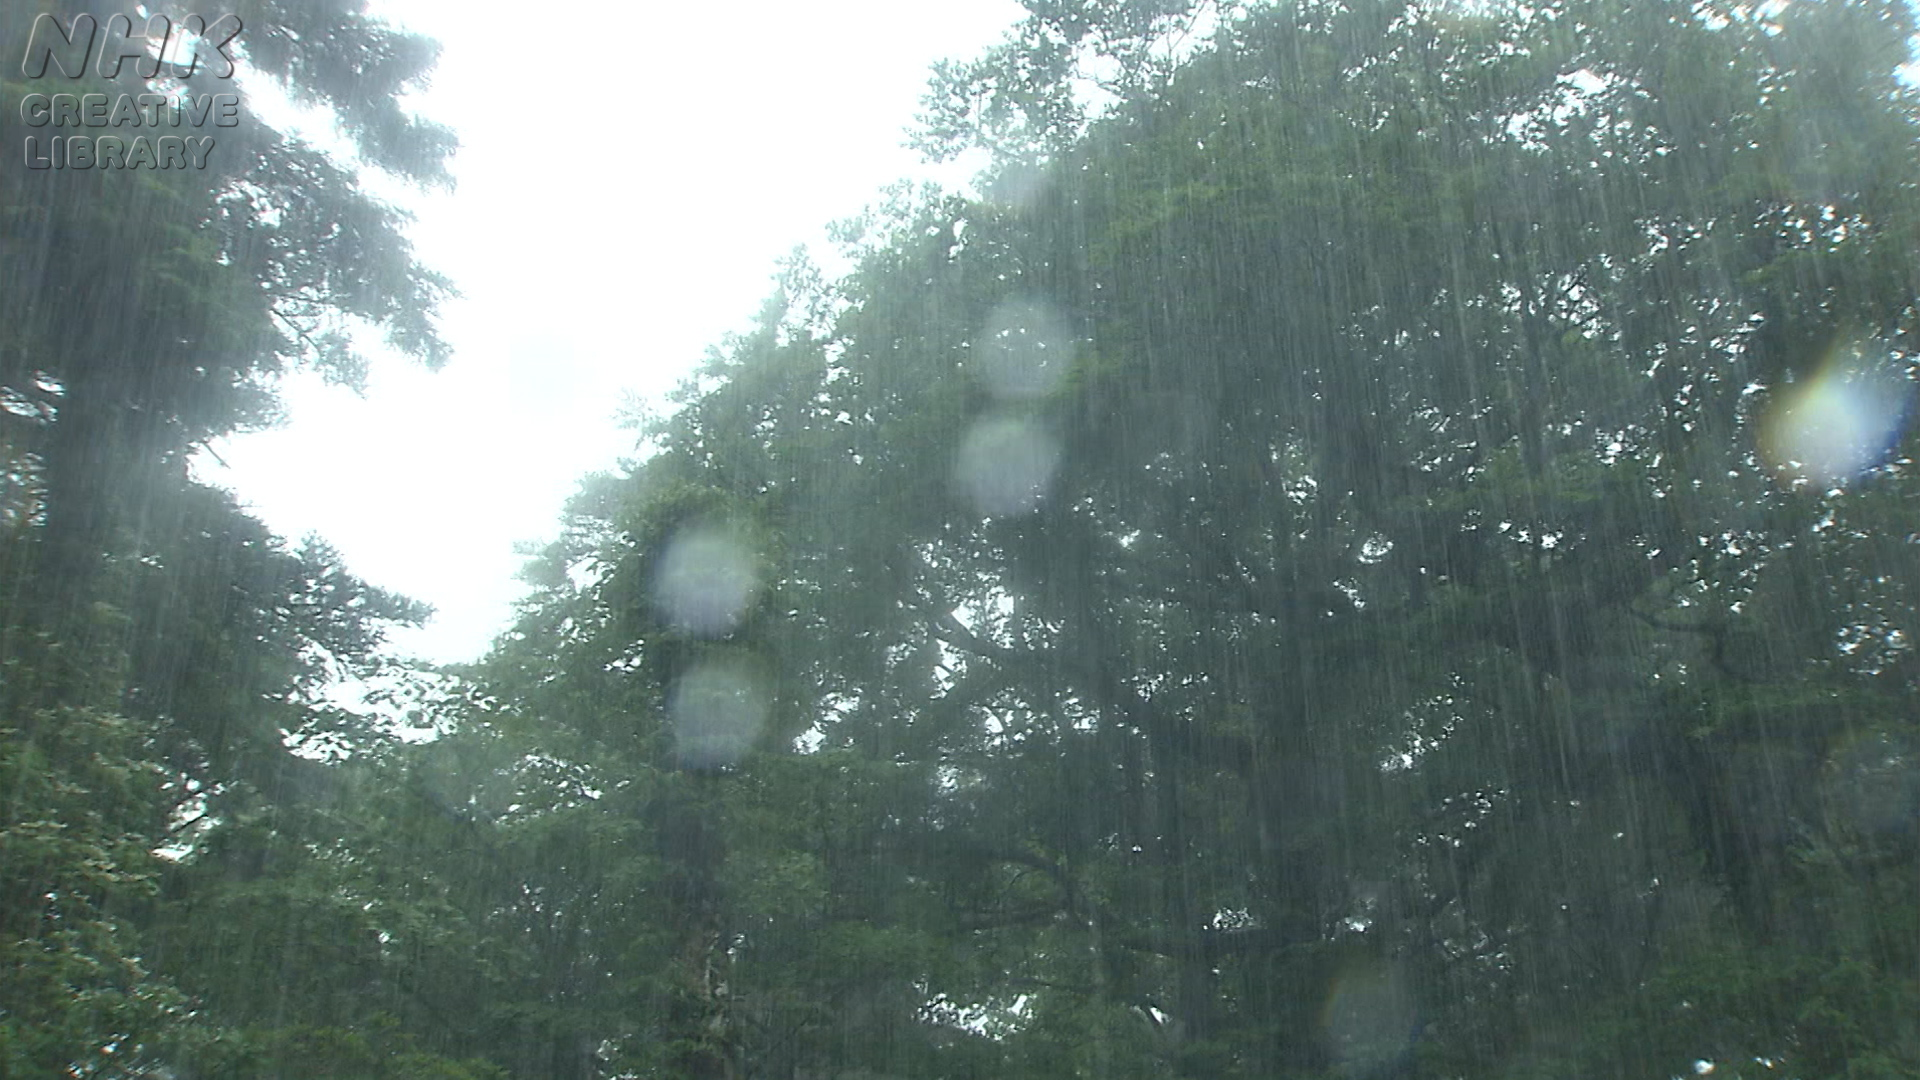
\includegraphics[width=8cm, height=4.5cm]{./fig/sample.jpg}%
	}{./movie/sample.mp4}
\end{frame}

\begin{frame}{外部ビューワーを呼び出し}
	\centering
	\movie[externalviewer]{
		Click to start the movie
	}{./movie/sample.mp4}
\end{frame}
\end{document}